\chapter{Le bloc p, I~: les groupes du bore, du carbone et de l'azote}\label{ch:b1:p-block-13-15}

L'air que nous respirons est constitué aux quatre cinquièmes de diazote,
et pourtant les plantes en manquent~: la triple liaison \ce{N#N} est si
forte que presque rien ne la rompt. Pendant l'essentiel de l'histoire,
l'azote des cultures est venu du fumier, de bactéries vivant sur les
racines des légumineuses et de nitrates extraits de mines. Au début du
vingtième siècle, une réaction entre le diazote et le dihydrogène sur un
\omterm{def:b1:elementary-steps:catalyst}{catalyseur} au fer a changé la donne~; le monde produit aujourd'hui
environ 160 millions de tonnes d'azote par an sous forme d'ammoniac, et
à peu près la moitié de l'azote d'un corps humain est passée par une
usine d'ammoniac. Les \omterm{def:b1:periodicity:table}{groupes} 13, 14 et 15 rassemblent les éléments de
cette histoire --- l'azote et le phosphore des engrais, le carbone et le
silicium de la vie et des roches, le bore et l'aluminium du verre et des
alliages légers. Ce chapitre les passe en revue avec les outils des
chapitres précédents.

\begin{recall}
Les \omterm{def:b1:crystals-metals:allotropy}{variétés allotropiques} du carbone et la structure du silicium et de
la silice (\cref{ch:b1:crystals-ionic-covalent})~; le caractère des
oxydes (\cref{def:b1:s-block:oxide-character})~; les \omterm{def:b1:nernst:oxidation-number}{nombres
d'oxydation} et les \omterm{def:b1:nernst:electrode-potential}{potentiels standard} (\cref{ch:b1:nernst})~; les
\omterm{def:b1:precipitation:amphoteric-hydroxide}{hydroxydes amphotères} (\cref{ch:b1:precipitation})~; les constantes
d'équilibre tirées des enthalpies libres
(\cref{ch:b1:extent-q-and-k}).
\end{recall}
% ledger: usgs:N-world-2025

\begin{omfigure}
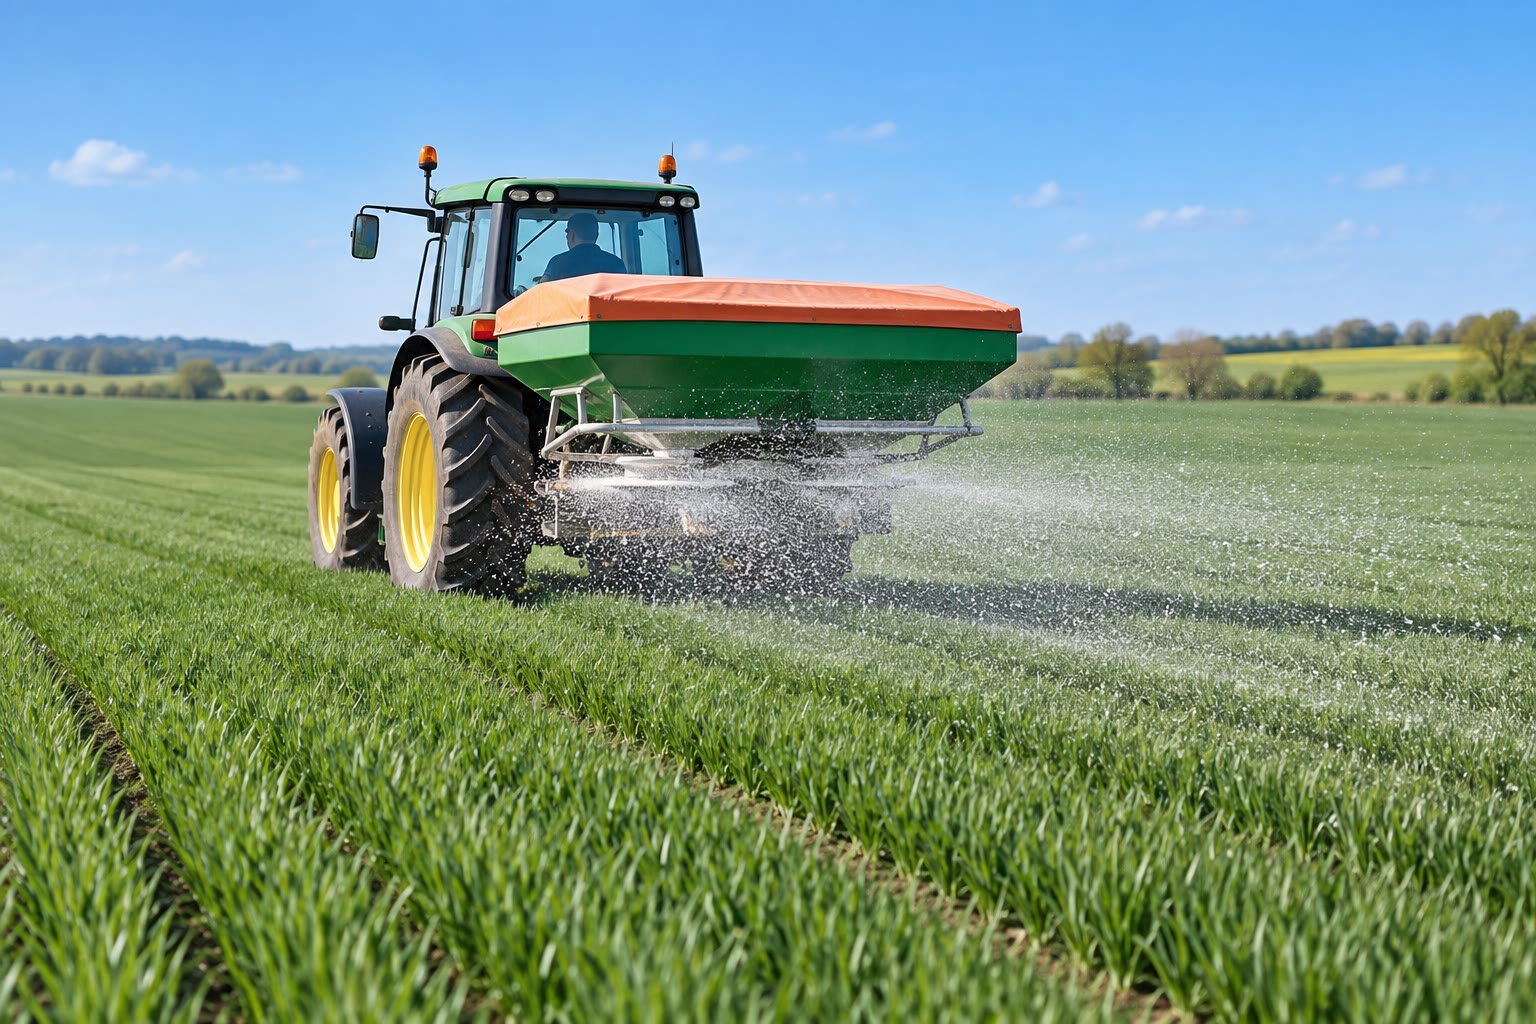
\includegraphics[width=0.55\linewidth]{images/book2/ai/b1-27-fertiliser-field.jpg}

{\small Épandage d'un engrais azoté sur un champ de blé. La plus grande
partie en a été fabriquée à partir de l'azote de l'air par le procédé
Haber--Bosch.}
\end{omfigure}

\section{Le groupe 13~: le bore et l'aluminium}

Le bore est un \omterm{def:b1:periodicity:metalloid}{métalloïde} qui forme des composés covalents à octet
incomplet~: dans \ce{BF3} et dans l'acide borique \ce{B(OH)3}, le bore a
six \omterm{def:b1:quantum-numbers:configuration}{électrons de valence} et se comporte en \omterm{def:b1:lewis-resonance-vsepr:lewis-acid}{acide de Lewis}
(\cref{ch:b1:lewis-resonance-vsepr}). L'acide borique est un \omterm{def:b1:predominant-reaction:strong-acid}{acide
faible} non parce qu'il perd un proton, mais parce qu'il accepte un ion
hydroxyde, \ce{B(OH)3 + 2H2O <=> B(OH)4- + H3O+}. Le borax, un borate de
sodium, est utilisé dans le verre et les détergents.

\begin{definition}[Oxoacide]\label{def:b1:p-block-13-15:oxoacid}
Un \emph{oxoacide}\index{oxoacide} est un acide dont les atomes
d'hydrogène acides sont liés à des atomes d'oxygène eux-mêmes liés à un
\omterm{def:b1:complexation:complex}{atome central}~:
\ce{B(OH)3}, \ce{H2CO3}, \ce{HNO3} (\ce{HO-NO2}), \ce{H3PO4}
(\ce{(HO)3PO}), \ce{H2SO4}. Plus l'\omterm{def:b1:complexation:complex}{atome central} est entouré d'atomes
d'oxygène dépourvus d'hydrogène, plus l'acide est fort.
\end{definition}

L'aluminium, sous le bore, est un métal, mais son ion petit et fortement
chargé lui donne un oxyde et un \omterm{def:b1:precipitation:amphoteric-hydroxide}{hydroxyde amphotères} (\cref{sec:b1:precipitation:amphoteric}).
Son minerai est la bauxite, mélange d'hydroxydes d'aluminium, d'oxydes de
fer et de silice~; en 2025, le monde a extrait environ 440 millions de
tonnes de bauxite et en a tiré environ 150 millions de tonnes d'alumine.
% ledger: usgs:bauxite-world-2025, usgs:alumina-world-2025

\begin{proposition}[Le procédé Bayer]\label{prop:b1:p-block-13-15:bayer}
L'hydroxyde de sodium concentré et chaud dissout l'aluminium de la
bauxite sous forme de
\ce{Al(OH)4-} et laisse les oxydes de fer (boues rouges)~; le
refroidissement et l'ensemencement de la solution filtrée font précipiter
du \ce{Al(OH)3} pur, calciné en alumine,
\ce{2Al(OH)3 -> Al2O3 + 3H2O}.
\end{proposition}

\begin{proof}
La réaction \ce{Al(OH)3(s) + OH- <=> Al(OH)4-} a pour constante $K = 10^{-1.23}$ à
\qty{25}{\celsius} (\cref{ch:b1:precipitation})~: lorsque \ce{[OH-]} est
élevée, l'aluminium est en solution, tandis que l'hydroxyde de fer(III),
qui n'est pas amphotère, reste solide (\cref{exo:b1:precipitation:12}).
La dilution et le refroidissement abaissent \ce{[OH-]} et modifient le
quotient de sorte que $Q > K$ pour la réaction inverse~: l'hydroxyde
précipite. La calcination élimine l'eau.
\end{proof}

L'alumine est ensuite réduite en aluminium par électrolyse dans la
cryolithe fondue, une industrie étudiée dans le volume de deuxième année.

\begin{omfigure}
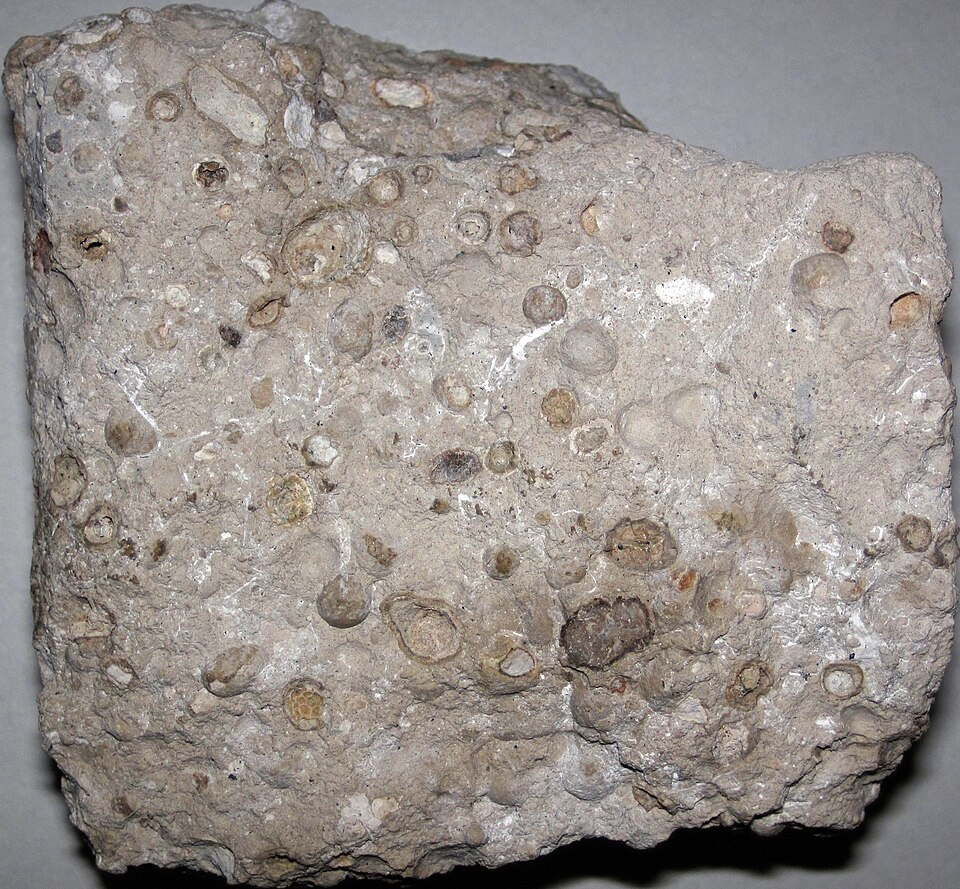
\includegraphics[height=3.6cm]{images/book2/bauxite.jpg}\hspace{0.4em}%
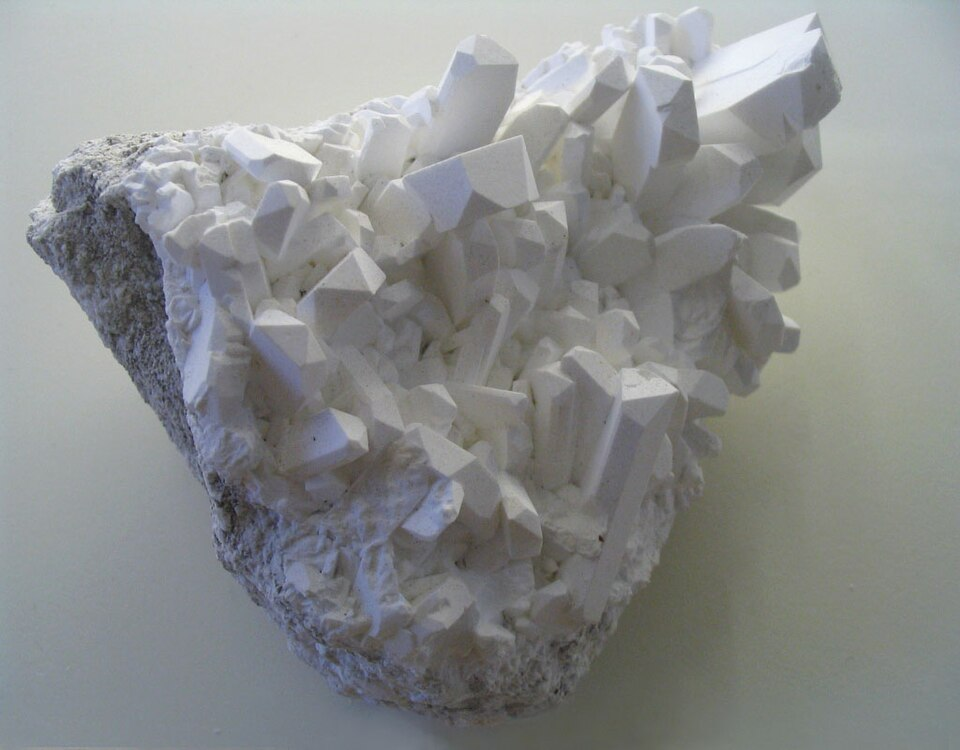
\includegraphics[height=3.6cm]{images/book2/borax.jpg}\hspace{0.4em}%
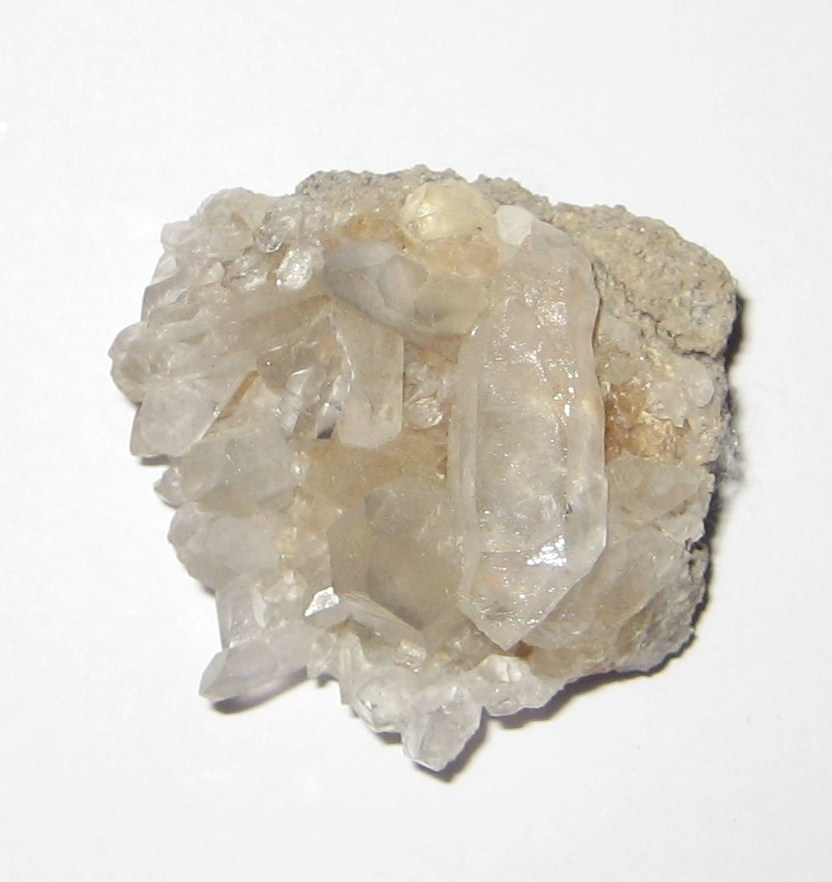
\includegraphics[height=3.6cm]{images/book2/quartz.jpg}\hspace{0.4em}%
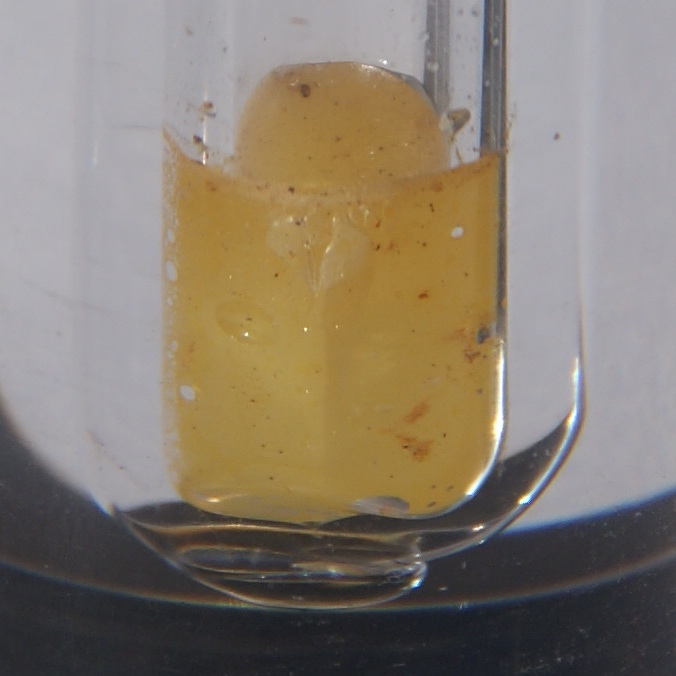
\includegraphics[height=3.6cm]{images/book2/white-phosphorus.jpg}

{\small De gauche à droite~: bauxite pisolithique (James St. John, CC BY 2.0)~;
\omterm{def:b1:crystals-metals:crystal}{cristaux} de borax (Aram Dulyan, domaine public)~; un amas de \omterm{def:b1:crystals-metals:crystal}{cristaux} de
quartz, \ce{SiO2} (Stephanie Clifford, CC BY 2.0)~; phosphore blanc,
avec un peu de phosphore rouge, conservé sous l'eau car il s'enflamme à
l'air (Hi-Res Images of Chemical Elements, CC BY 3.0). Toutes les images
proviennent de Wikimedia Commons.}
\end{omfigure}

\section{Le groupe 14~: le carbone et le silicium}

Le carbone et le silicium forment tous deux quatre liaisons, mais
différemment. Le carbone forme de fortes doubles liaisons~: \ce{CO2} est
une molécule, \ce{O=C=O}, un gaz. Le silicium n'en forme guère~:
\ce{SiO2} est un réseau covalent de tétraèdres \ce{SiO4} qui partagent
tous leurs sommets, un solide dur, le quartz (\cref{ch:b1:crystals-ionic-covalent}).
Le dioxyde de carbone est un \omterm{def:b1:s-block:oxide-character}{oxyde acide}, qui donne l'acide carbonique,
les hydrogénocarbonates et les carbonates
(\cref{ch:b1:predominant-reaction})~; la silice est elle aussi un \omterm{def:b1:s-block:oxide-character}{oxyde
acide}, attaqué par les alcalis fondus en donnant des silicates.

\begin{proposition}[Les motifs silicatés]\label{prop:b1:p-block-13-15:silicate-units}
Les silicates sont construits à partir de tétraèdres \ce{SiO4}~; le
nombre de sommets partagés avec d'autres tétraèdres fixe la formule de
l'anion~: aucun, \ce{SiO4^4-}
(tétraèdres isolés)~; deux, chaînes $(\ce{SiO3})_n^{2n-}$~; trois,
feuillets
$(\ce{Si2O5})_n^{2n-}$~; quatre, la charpente neutre \ce{SiO2}.
\end{proposition}

\begin{proof}
Un oxygène partagé appartient pour moitié à chaque tétraèdre. Un
tétraèdre qui partage
$k$ sommets possède entièrement $4 - k$ atomes d'oxygène et $k$ pour
moitié~: $4 -
k/2$ oxygènes par silicium. Chaque oxygène non partagé porte une charge
$-1$ (il n'a qu'une liaison), chaque oxygène partagé aucune~: la charge
par silicium vaut
$-(4 - k)$. $k = 0$~: \ce{SiO4^4-}~; $k = 2$~: \ce{SiO3^2-} par
silicium~;
$k = 3$~: \ce{SiO_{2.5}^-}, c'est-à-dire \ce{Si2O5^2-}~; $k = 4$~: \ce{SiO2}.
\end{proof}

\begin{omfigure}
\begin{tikzpicture}[font=\small, line join=round]
  % one SiO4 tetrahedron in perspective
  \begin{scope}
    \coordinate (t) at (0,1.2); \coordinate (a) at (-1.0,-0.5);
    \coordinate (b) at (1.0,-0.5); \coordinate (c) at (0.25,0.05);
    \draw[thick, omDef] (t) -- (a) -- (b) -- cycle; \draw[thick, omDef] (t) -- (b);
    \draw[dashed, omDef] (a) -- (c) -- (b) (t) -- (c);
    \foreach \p in {t,a,b,c} \shade[ball color=red!60] (\p) circle (0.16);
    \shade[ball color=gray!40] (0.06,0.18) circle (0.11);
    \node at (0,-1.2) {\ce{SiO4^4-}~: un tétraèdre};
  \end{scope}
  % a chain of tetrahedra seen from above
  \begin{scope}[xshift=3.6cm]
    \foreach \i in {0,1,2,3} {
      \draw[thick, omDef, fill=omDef!10] (\i*1.1,0) -- (\i*1.1+0.55,0.95) -- (\i*1.1+1.1,0) -- cycle;
      \shade[ball color=red!60] (\i*1.1+0.55,0.95) circle (0.12);
      \shade[ball color=red!60] (\i*1.1+0.55,0.32) circle (0.10);
    }
    \foreach \i in {0,1,2,3,4} \shade[ball color=red!60] (\i*1.1,0) circle (0.12);
    \node[align=center] at (2.2,-1.0) {chaîne $(\ce{SiO3})_n^{2n-}$~: chaque tétraèdre\\ partage deux sommets (vue de dessus)};
  \end{scope}
\end{tikzpicture}

{\small Motifs silicatés~: un tétraèdre \ce{SiO4} isolé (silicium en
gris, oxygène en rouge), et une chaîne dans laquelle chaque tétraèdre
partage deux atomes d'oxygène avec ses voisins. Les feuillets (trois
sommets partagés) forment les micas et les argiles~; une charpente
(quatre) forme le quartz.}
\end{omfigure}

\begin{definition}[Effet de paire inerte]\label{def:b1:p-block-13-15:inert-pair}
L'\emph{effet de paire inerte}\index{effet de paire inerte} est la
stabilité croissante, en descendant les \omterm{def:b1:periodicity:table}{groupes} 13 à 15, du degré
d'oxydation inférieur de deux au degré maximal du groupe~: thallium(I)
plutôt que (III), plomb(II) plutôt que (IV), bismuth(III) plutôt que
(V). Le doublet \textit{ns}$^2$ des éléments lourds est fortement retenu
et participe peu aux liaisons.
\end{definition}

Cet effet explique pourquoi l'oxyde de plomb(IV) est un \omterm{def:b1:nernst:couple}{oxydant} fort
($E^\circ(\ce{PbO2}/\ce{Pb^2+}) = 1.46$~V, \cref{ch:b1:nernst}), alors que
le carbone(IV) et le silicium(IV) sont les états stables de leurs
éléments.

\section{Le groupe 15~: l'azote}

\begin{proposition}[L'échelle de l'azote]\label{prop:b1:p-block-13-15:nitrogen-ladder}
L'azote prend tous les \omterm{def:b1:nernst:oxidation-number}{nombres d'oxydation} de $-3$ à $+5$~: \ce{NH3} et
\ce{NH4+} ($-$III), \ce{N2H4} ($-$II), \ce{NH2OH} ($-$I), \ce{N2} (0),
\ce{N2O} ($+$I), \ce{NO} ($+$II), \ce{HNO2} et \ce{NO2-} ($+$III),
\ce{NO2} ($+$IV), \ce{HNO3} et \ce{NO3-} ($+$V).
\end{proposition}

\begin{proof}
Appliquer les règles de la \cref{prop:b1:nernst:on-rules} à chaque
formule, avec H à $+$I et O à $-$II~: dans \ce{N2H4}, $2x + 4 = 0$~;
dans \ce{NO2-}, $x - 4 =
-1$~; et ainsi de suite.
\end{proof}

\begin{definition}[Fixation de l'azote]\label{def:b1:p-block-13-15:nitrogen-fixation}
La \emph{fixation de l'azote}\index{fixation de l'azote} désigne tout
processus qui convertit le diazote de l'air en un composé (ammoniac,
nitrate) utilisable par les êtres vivants ou par l'industrie~: fixation
biologique par des bactéries, fixation par la foudre, et synthèse
industrielle de l'ammoniac.
\end{definition}

Le procédé Haber--Bosch combine le diazote et le dihydrogène sur un
\omterm{def:b1:elementary-steps:catalyst}{catalyseur} au fer, \ce{N2 + 3H2 <=> 2NH3}. La réaction est favorisée à
température ambiante ($K = 10^{5.8}$ à \qty{25}{\celsius}, d'après
l'enthalpie libre de formation de l'ammoniac), mais trop lente~; le
\omterm{def:b1:elementary-steps:catalyst}{catalyseur} n'agit qu'à chaud, et le choix de la température et de la
pression qui concilie vitesse et \omterm{def:b1:extent-q-and-k:fractional-extent}{rendement} est fait dans le volume de
deuxième année. L'ammoniac est ensuite oxydé en acide nitrique par le
procédé Ostwald.
% ledger: dfg:NH3_g

\begin{omfigure}
\begin{tikzpicture}[font=\small, >={Stealth}, box/.style={draw, rounded corners, fill=omDef!8, align=center, minimum height=0.9cm}]
  \node[box] (air) at (0,0) {air\\\ce{N2}};
  \node[box] (gas) at (0,-1.6) {gaz naturel\\\ce{H2}};
  \node[box] (hb) at (3.4,-0.8) {Haber--Bosch\\catalyseur au fer};
  \node[box] (ox1) at (7.3,-0.8) {toile Pt--Rh\\\ce{NH3} $\to$ \ce{NO}};
  \node[box] (ox2) at (11.0,-0.8) {oxydation\\absorption\\\ce{NO} $\to$ \ce{NO2} $\to$ \ce{HNO3}};
  \draw[->, thick] (air) -- (hb);
  \draw[->, thick] (gas) -- (hb);
  \draw[->, thick] (hb) -- node[above] {\ce{NH3}} (ox1);
  \draw[->, thick] (ox1) -- node[above] {\ce{NO}} (ox2);
  \draw[->, thick] (ox2.south) -- ++(0,-0.6) node[below] {\ce{HNO3}};
  \draw[->, thick] (hb.south) -- ++(0,-0.9) node[below] {\ce{NH3} (engrais)};
  \draw[->, thick] (ox2.north) -- ++(0,0.5) -| node[pos=0.25, above] {\ce{NO} recyclé} (ox1.north);
\end{tikzpicture}

{\small De l'air à l'acide nitrique~: la synthèse de l'ammoniac suivie
des trois étapes du procédé Ostwald.}
\end{omfigure}

\begin{method}[Équilibrer des équations industrielles enchaînées]\label{met:b1:p-block-13-15:ostwald-balance}
\begin{enumerate}
  \item Équilibrer chaque étape~: (1) \ce{4NH3 + 5O2 -> 4NO + 6H2O}~;
        (2) \ce{2NO + O2 -> 2NO2}~; (3) \ce{3NO2 + H2O -> 2HNO3 + NO}.
  \item Multiplier les étapes de sorte que chaque intermédiaire formé
        soit consommé (le \ce{NO} de l'étape 3 retourne à l'étape 2).
  \item Additionner~: avec un recyclage complet de NO, l'équation globale
        est
        \ce{NH3 + 2O2 -> HNO3 + H2O}, un acide nitrique par ammoniac.
  \item Utiliser l'équation globale pour les bilans de matière, les
        étapes pour la conception de chaque réacteur.
\end{enumerate}
\end{method}

\begin{history}[Fritz Haber]
\begin{minipage}[t]{0.18\linewidth}\vspace{0pt}
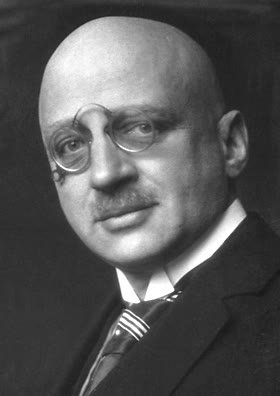
\includegraphics[width=\linewidth]{images/book2/haber.jpg}
\end{minipage}\hfill
\begin{minipage}[t]{0.78\linewidth}\vspace{0pt}
Fritz Haber montra que l'on pouvait fabriquer l'ammoniac à partir du
diazote et du dihydrogène sous pression, sur un \omterm{def:b1:elementary-steps:catalyst}{catalyseur}~; Carl Bosch
fit de la réaction de laboratoire un procédé industriel. Haber reçut le
prix Nobel de chimie de 1918. Le même homme dirigea le premier emploi à
grande échelle du dichlore comme arme, pendant la Première Guerre
mondiale~: la chimie qui nourrit la moitié de l'humanité et celle qui
tue ne sont séparées que par les choix des chimistes. (Photographie~:
The Nobel Foundation, publiée en 1919, domaine public, Wikimedia
Commons.)
\end{minipage}
\end{history}

\section{Le phosphore et les évolutions le long des groupes}

Le phosphore, sous l'azote, ne forme pas de triples liaisons \ce{P#P}~:
le phosphore blanc est constitué de tétraèdres \ce{P4}, tendus et
réactifs (il s'enflamme à l'air et se conserve sous l'eau)~; le
phosphore rouge est un polymère, bien moins réactif. La combustion du
phosphore donne \ce{P4O10}, le plus acide des oxydes courants, qui donne
avec l'eau l'acide phosphorique,
$\mathrm{p}K_a$ 2.15, 7.21, 12.34 (\cref{ch:b1:predominant-reaction}).
Les phosphates naturels, extraits à raison d'environ 250 millions de
tonnes en 2025, sont transformés en engrais phosphatés par l'acide
sulfurique.
% ledger: usgs:phosphate-world-2025

En descendant chaque groupe, les éléments deviennent plus métalliques
(du bore au thallium, du carbone au plomb, de l'azote au bismuth), leurs
oxydes plus basiques, et les degrés d'oxydation inférieurs plus
stables~: c'est l'\omterm{def:b1:p-block-13-15:inert-pair}{effet de paire inerte}. Le long d'une \omterm{def:b1:periodicity:table}{période}, les
oxydes deviennent plus acides, de \ce{Na2O}, basique, aux \omterm{def:b1:s-block:oxide-character}{oxydes acides}
du phosphore et du soufre.

\section{Exercices}

\begin{exercise}[$\star$]\label{exo:b1:p-block-13-15:1}
Donner le \omterm{def:b1:nernst:oxidation-number}{nombre d'oxydation} de l'azote dans \ce{NH4NO3} (les deux
atomes),
\ce{N2O5}, \ce{HNO2}, \ce{N2H4} et \ce{Mg3N2}.
\end{exercise}

\begin{exercise}[$\star$]\label{exo:b1:p-block-13-15:2}
Dessiner les \omterm{def:b1:lewis-resonance-vsepr:lewis}{schémas de Lewis} de \ce{BF3}, de \ce{NH3} et de l'adduit
\ce{F3B-NH3}~; identifier l'acide et la \omterm{def:b1:lewis-resonance-vsepr:lewis-acid}{base de Lewis}.
\end{exercise}

\begin{exercise}[$\star$]\label{exo:b1:p-block-13-15:3}
Écrire les réactions de \ce{CO2}, de \ce{SiO2} (fondue) et de
\ce{P4O10} avec l'hydroxyde de sodium, et de \ce{Al2O3} avec un acide et
avec une base.
\end{exercise}

\begin{exercise}[$\star$]\label{exo:b1:p-block-13-15:4}
Calculer la constante d'équilibre de \ce{N2 + 3H2 <=> 2NH3} à
\qty{25}{\celsius} à partir de $\Delta_f G^\circ(\ce{NH3}) =
\qty{-16.45}{kJ/mol}$.
\end{exercise}

\begin{exercise}[$\star\star$]\label{exo:b1:p-block-13-15:5}
À l'aide du décompte de la \cref{prop:b1:p-block-13-15:silicate-units},
donner la formule d'un cycle de six tétraèdres partageant chacun deux
sommets (comme dans le béryl) et celle d'une chaîne double dans laquelle
la moitié des tétraèdres partagent deux sommets et l'autre moitié trois.
\end{exercise}

\begin{exercise}[$\star\star$]\label{exo:b1:p-block-13-15:6}
Calculer la masse d'alumine obtenue à partir d'une tonne de bauxite
contenant \qty{55}{\percent} en masse de \ce{Al(OH)3}, avec un taux de
récupération de \qty{92}{\percent}.
\end{exercise}

\begin{exercise}[$\star\star$]\label{exo:b1:p-block-13-15:7}
Montrer que l'acide borique est un \omterm{def:b1:lewis-resonance-vsepr:lewis-acid}{acide de Lewis} plutôt qu'un \omterm{def:b1:predominant-reaction:bronsted}{acide de
Brønsted}, et expliquer pourquoi sa solution est néanmoins acide.
\end{exercise}

\begin{exercise}[$\star\star$]\label{exo:b1:p-block-13-15:8}
Équilibrer l'oxydation de l'ammoniac en \ce{NO} à l'aide des \omterm{def:b1:nernst:oxidation-number}{nombres
d'oxydation} et donner le nombre d'électrons échangés par \ce{NH3}.
\end{exercise}

\begin{exercise}[$\star\star$]\label{exo:b1:p-block-13-15:9}
Le nitrate d'ammonium est fabriqué à partir d'ammoniac et d'acide
nitrique. Écrire la réaction, et calculer la masse d'ammoniac nécessaire
(à la fois pour l'acide nitrique et pour la neutralisation) par tonne de
nitrate d'ammonium.
\end{exercise}

\begin{exercise}[$\star\star\star$]\label{exo:b1:p-block-13-15:10}
Expliquer pourquoi l'azote est un gaz diatomique et le phosphore un
solide de molécules \ce{P4}, et pourquoi le dioxyde de carbone est un
gaz et la silice un solide, à l'aide de la force des liaisons $\pi$
entre atomes de la deuxième et de la troisième \omterm{def:b1:periodicity:table}{période}.
\end{exercise}

\begin{exercise}[$\star\star\star$]\label{exo:b1:p-block-13-15:11}
Montrer à l'aide des \omterm{def:b1:nernst:electrode-potential}{potentiels standard} que l'oxyde de plomb(IV) oxyde
les ions chlorure en dichlore en milieu acide, alors que l'oxyde de
silicium(IV) n'a rien de tel. Relier ce résultat à l'\omterm{def:b1:p-block-13-15:inert-pair}{effet de paire
inerte}.
\end{exercise}

\begin{exercise}[$\star\star\star$]\label{exo:b1:p-block-13-15:12}
Le monde a produit environ 160 millions de tonnes d'azote sous forme
d'ammoniac en 2025. Quelle masse d'ammoniac cela représente-t-il, et
quelle masse d'hydrogène contenait-elle~? D'où provient surtout cet
hydrogène~?
\end{exercise}

\section{Problème~: de l'air aux engrais}

\begin{problem}[{Problème du week-end --- la triple liaison de l'azote,
la synthèse de l'ammoniac, les trois étapes de la fabrication de l'acide
nitrique, le nitrate d'ammonium, et la masse d'acide nitrique que l'on
peut obtenir à partir d'une tonne d'ammoniac}]
\label{pb:b1:p-block-13-15:1}
Une usine d'engrais convertit l'ammoniac en acide nitrique et en nitrate
d'ammonium. Masses molaires (\unit{g/mol})~: \ce{N2} 28.0, \ce{H2} 2.0, \ce{NH3}
17.0, \ce{HNO3} 63.0, \ce{NH4NO3} 80.0, \ce{O2} 32.0~;
$\Delta_f G^\circ(\ce{NH3(g)}) = \qty{-16.45}{kJ/mol}$ à
\qty{25}{\celsius}.

\medskip
\noindent\textbf{Partie I --- L'azote.}
\begin{enumerate}
  \item Dessiner le \omterm{def:b1:lewis-resonance-vsepr:lewis}{schéma de Lewis} de \ce{N2} et dire pourquoi il est peu
        réactif.
  \item Donner le \omterm{def:b1:nernst:oxidation-number}{nombre d'oxydation} de N dans \ce{N2}, \ce{NH3}, \ce{NO},
        \ce{NO2}, \ce{HNO3} et \ce{NH4NO3}.
  \item Citer trois voies, naturelles ou industrielles, de \omterm{def:b1:p-block-13-15:nitrogen-fixation}{fixation de
        l'azote}.
  \item Pourquoi les plantes ne peuvent-elles pas utiliser directement
        \ce{N2}~?
  \item Quel élément est oxydé et lequel est réduit lors de la synthèse
        de l'ammoniac~?
  \item Écrire la synthèse de l'ammoniac.
\end{enumerate}

\medskip
\noindent\textbf{Partie II --- L'ammoniac.}
\begin{enumerate}[resume]
  \item Calculer la constante d'équilibre de la synthèse à
        \qty{25}{\celsius}.
  \item Pourquoi la synthèse est-elle néanmoins menée à chaud, sur un
        \omterm{def:b1:elementary-steps:catalyst}{catalyseur}~?
  \item Calculer les masses de \ce{N2} et de \ce{H2} pour une tonne
        d'ammoniac.
  \item Quel volume d'air (\qty{78}{\percent} de \ce{N2} en volume, gaz
        parfait, \qty{25}{\celsius}, \qty{1}{bar}) contient ce diazote~?
  \item D'où vient le dihydrogène~?
  \item Pourquoi l'ammoniac lui-même est-il utilisé comme engrais dans
        certains pays, et pourquoi est-il souvent d'abord converti~?
\end{enumerate}

\medskip
\noindent\textbf{Partie III --- L'acide nitrique.}
\begin{enumerate}[resume]
  \item Équilibrer l'étape 1, \ce{NH3 + O2 -> NO + H2O}, à l'aide des \omterm{def:b1:nernst:oxidation-number}{nombres d'oxydation}. % ce-unbalanced-ok
  \item Équilibrer l'étape 2, \ce{NO + O2 -> NO2}. % ce-unbalanced-ok
  \item Équilibrer l'étape 3, \ce{NO2 + H2O -> HNO3 + NO}. De quel type % ce-unbalanced-ok
        de réaction d'oxydoréduction s'agit-il~?
  \item Combiner les étapes, avec un recyclage complet de NO, en
        l'équation globale.
  \item Calculer la masse de dioxygène consommée par tonne d'ammoniac.
  \item Pourquoi utilise-t-on une toile de platine--rhodium à l'étape 1~?
\end{enumerate}

\medskip
\noindent\textbf{Partie IV --- Le nitrate d'ammonium et les bilans de matière.}
\begin{enumerate}[resume]
  \item Écrire la formation du nitrate d'ammonium.
  \item Quelle fraction de l'ammoniac doit être transformée en acide
        nitrique pour ne fabriquer que du nitrate d'ammonium~?
  \item Calculer la masse de nitrate d'ammonium obtenue à partir d'une
        tonne d'ammoniac répartie de cette façon.
  \item Quel pourcentage d'azote le nitrate d'ammonium contient-il~?
  \item Pourquoi faut-il stocker le nitrate d'ammonium à l'écart des
        combustibles et de la chaleur~?
  \item Calculer la masse d'acide nitrique que l'on peut obtenir à partir
        d'une tonne d'ammoniac (conversion complète).
\end{enumerate}
\end{problem}
